\documentclass{beamer}
\usepackage[utf8]{inputenc}
\usepackage{xcolor}
\usepackage{listings}
\usepackage{graphicx}
\usetheme[secheader]{Boadilla}
\definecolor{coultitre}{rgb}{0,0.65,0}
\setbeamercolor{structure}{fg=coultitre, bg=coultitre!40} 





\title{Vidéo surveillance, Streaming vidéo et contrôle de caméra via Android }
\author{\tiny{Jérôme NAHELOU, Quentin NEBOUT, Romain SOLVE, Fabien QUINTARD}}

\institute{\large{Chargé de Projet : Yérom-David Bromberg}\\ \bigskip{}

\small{Université Bordeaux 1}}
\date{29 mars 2011}


\begin{document}
\frame[plain]{\titlepage}

\AtBeginSection[]{
\begin{frame}<beamer>
\frametitle{Plan}
\tableofcontents[hideallsubsections,currentsection]
\end{frame}}

\begin{frame}
\frametitle{Plan de l'exposé}
\tableofcontents[hideallsubsections]
\end{frame}


  \begin{frame}
   \frametitle{Description}
  Introduction
  % schéma projet : dessin camera + portablets et tablettes android en réseau %
   \begin{itemize}
    \item Android: OS pour appareil mobile, basé sur noyaux linux
    \item Choix: M-JPEG, HTTP-GET
   \end{itemize}
  \end{frame}
  
  \begin{frame}
   \frametitle{Besoins}
  Introduction
  % schéma besoins F / besoins NF %
  \end{frame}

\section{Aspect général de l'application}
  \subsection{Description}
  \begin{frame}
   \frametitle{Description}
  Aspect général de l'application convivial
   \begin{itemize}
    \item Astuces pour mieux connaître les fonctionnalités
    \item Application Multi-langue avec détection automatique
   \end{itemize}
  \end{frame}

\section{Simple vue}
\subsection{Spécifications}
 \begin{frame}
   \frametitle{Spécifications}
   \begin{itemize}
    \item Réutilisation d'un lecteur MJPEG existant : MjpegView
    \item Interface de contrôle de la caméra
    % screen simple vue %
    \end{itemize}
\end{frame}

\section{Multi-vue}
\subsection{Spécifications}
 \begin{frame}
   \frametitle{Spécifications}
   \begin{itemize}
    \item Implémentation de layouts personnalisés pour 2 à 6 caméras
    % schéma ou screen multi-vue %
    \item Rafraîchissement multi-threadé (un thread par caméra)
    % schéma UML de Jérôme ;) %
    \item Ajout de listeners pour gérer les caméras et passer en simple vue 
    \end{itemize}
\end{frame}

\section{Contrôle de la caméra}
\subsection{Implémentation}
 \begin{frame}
   \frametitle{Implémentation}
   \begin{itemize}
    \item Communication avec la caméra par requêtes HTTP
    \item Chargement de la configuration à l'initialisation de la vidéo
    \item Méthode de construction et d'envoi des requêtes avec
    authentification et délai variable de connexion
   \end{itemize}
\end{frame}

\subsection{Interfaces}
 \begin{frame}
\frametitle{Interfaces}
   Plusieurs interfaces de contrôle direct :
   \begin{itemize}
    \item Flux vidéo en continu pour actions en temps réel
    \item Contrôle du Pan/Tilt/Zoom de manière tactile
    % schéma notion tactile %
    \item Interface de commandes avancées adaptée à la caméra
    \item Module de gestion de détection de mouvements
   \end{itemize}
\end{frame}

\section{Détection de mouvements}
\subsection{Principe Axis}
 \begin{frame}
   \frametitle{Pricipe Axis}
    Le mécanisme de la détection de mouvements par Axis est le suivant :
   \begin{itemize}
    \item Ajout d'une fenêtre de détection spécifique (coordonnées,
    sensibilité, \ldots) par l'utilisateur
    \item Solution 1 : Ajout d'un événement déclenché automatiquement à la
    présence d'un mouvement (email, SMS, \ldots)
    \item Solution 2 : Demande du flux de niveaux de détection pour un
    calcul et un traitement personnalisés
   \end{itemize}
\end{frame}

\subsection{Implémentation Android}
 \begin{frame}
   \frametitle{Implémentation Android}
    La solution 2 a été retenue pour notre application :
    \begin{itemize}
    \item Définition de la fenêtre directement sur l'écran (composant
    graphique)
    \item Mise en arrière-plan du thread de calcul (utilisation d'un service
    Android)
    \item Alerte par notification : vibration + snapshot
    % deuxième schéma UML de Jérôme %
   \end{itemize}
\end{frame}

\section{Tests}
\subsection{Tests Unitaires}
  \begin{frame}
\begin{minipage}{0.32\textwidth}
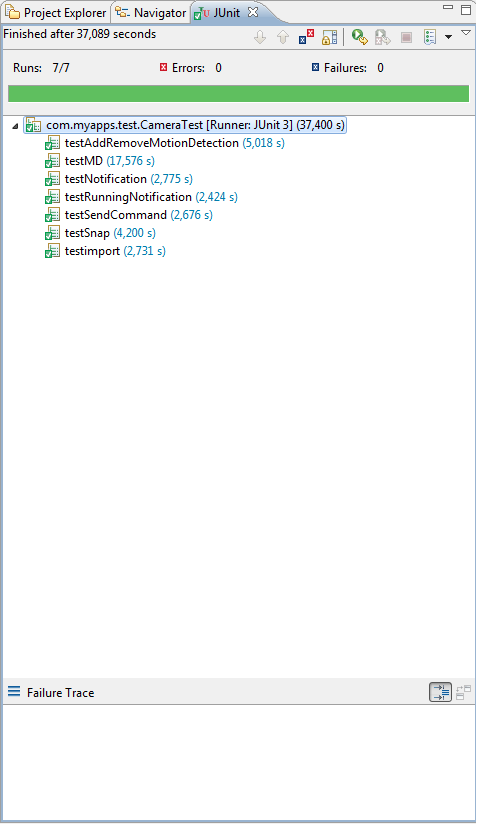
\includegraphics[width=3.5cm, height=7cm]{Images/ImageSlide12a.png}
\end{minipage}
\begin{minipage}{0.49\textwidth}
\frametitle{Tests Unitaires}
Rôle des tests unitaires
  \begin{itemize}
 \item Garantir le bon fonctionnement de l'application
    \item Vérifier si les fonctions terminent
    \item Identifier étape par étape les erreurs éventuelles
\end{itemize} 
\end{minipage}
\begin{minipage}{0.10\textwidth}
 
\includegraphics[width=3cm, height=2.2cm]{Images/ImageSlide12.png}
\end{minipage}
\end{frame}

\subsection{Tests en réel}
 \begin{frame}
\begin{minipage}{0.59\textwidth}
   \frametitle{Tests en réel}
\begin{itemize}
    \item Suivi de l'exécution en continu avec le LogCat d'Android
    \item Utilisation intensive de 3 téléphones de marques différentes
    \item Tests sur une caméra Axis PTZ 214 avec l'ensemble des
    fonctionnalités implémentées
   \end{itemize}
\end{minipage}
\begin{minipage}{0.39\textwidth}
 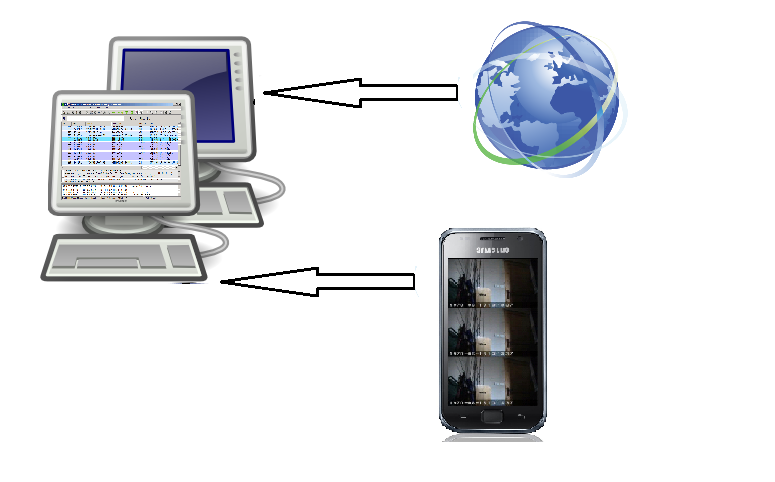
\includegraphics[width=4cm, height=3cm]{Images/ImageSlide13.png}
\end{minipage}
\end{frame}




\subsection{Optimisations}
 \begin{frame}
   \frametitle{Optimisations}

\end{frame}


\section{Vue Multiple}
  \subsection{Analyse du besoin}
  \begin{frame}
   \frametitle{Analyse du besoin}


\begin{figure}[H]
  \centering
  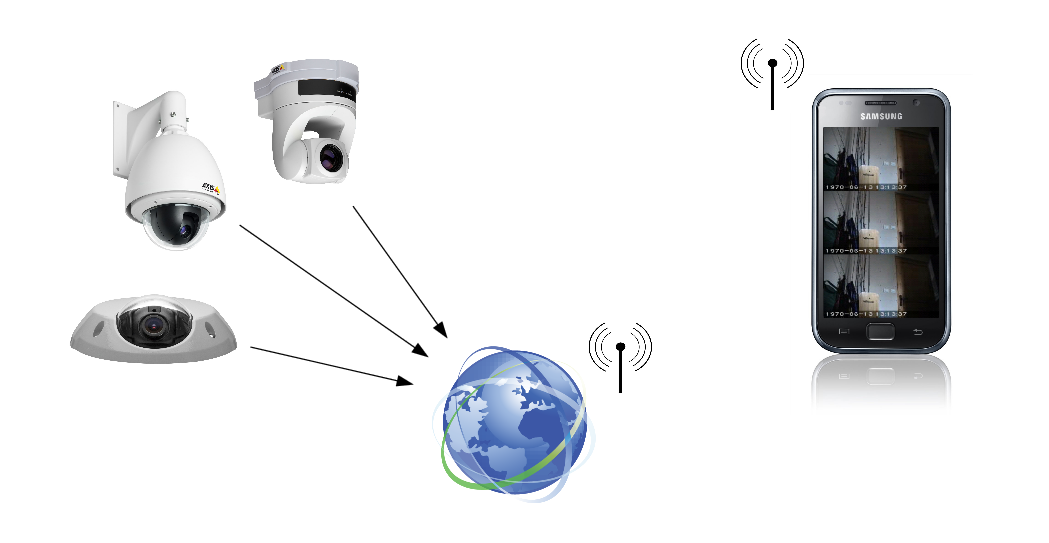
\includegraphics[scale=0.25]{Images/ImageSlide9.png}
     \begin{itemize}
    \item Possibilité de visionner 1 à 6 Caméras simultanément
    \item Choix de la disposition des caméras par l'utilisateur
    \item Réglage du nombre d'images par seconde
    \item Switch ``Multiple-Vue" - ``Vue unitaire"
   \end{itemize}
  \end{figure}  

\end{frame}


\end{document}